\chapter{Experiments and Numerical Results}
\label{chap:results}
%\minitoc

\section{Instances of VRPSD}

To compare results we are used instances of two diferents sources, the first set of instances was generated following a procedure similar to the used in Secomandi~\cite{secomandi_comparing_2000}, the another set of instances is the used by Novoa ~\cite{novoa_approximate_2009}, Both instance sets are generated using the procedure described on the next section.

\subsection{Instance generation}

The set of instances contain 45 different instances resulting from combine three number of customers $n \in \{5,10,20\}$, three vehicle capacities given for $f'$ factor and five different assignments for customer locations and demand distribution for each one, the assignments result from changing the random seeds.

The customers' demands are both discrete and distributed uniformly in this posible sets $U[1,5]$, $U[3,9]$, $U[6,12]$, in each instance, each customer is assigned to any of the three groups with equal probability. Customers' locations are random points in $[0, 1]^2$, with the depot fixed at $(0,0)$.%, e.g. figure \ref{fig:instance_n5_f1_s1}.

%\begin{figure}[h]
  % Requires \usepackage{graphicx}
%  \includegraphics[scale=0.4]{images/n5_f1_s1}\\
%  \caption{Customers' location, n = 5}\label{fig:instance_n5_f1_s1}
%\end{figure}

The filling rate $f$ is an index of the total expected demand relative to vehicle capacity.

\begin{equation}\label{eq:4filling-rate}
f=\sum_{i=1}^n\frac{E[D_i]}{mQ}
\end{equation}

where $E[D_i]$ is the expected demand of customer $i$, $m$ is the number of available vehicles, when $m = 1$ $f$ can represent approximately the expected number of replenishment needed to serve all customers' demands. It follows that, a priori, in all instances $E[D_i]=(3+6+9)/3=6$, for any customer i, and $Q=6n/f$. $f'=f-1$ is the expected number of route failure in a given instance. Hence, we is defined for this factor $f' \in \{1.0, 1.5, 2.0\}$, following the same factors used by Secomandi~\cite{secomandi_comparing_2000}.

\begin{table}
  \centering
  \caption{Vehicle capacity for each factor}\label{tb:Q}
\begin{tabular}{l l l l}
  \hline
  % after \\: \hline or \cline{col1-col2} \cline{col3-col4} ...
  $f'$ &   & $n$ &   \\
  \cline{2-4}
      & 5 & 10 & 15 \\
  \hline
  1.0 & 15 & 30 & 45 \\
  1.5 & 12 & 24 & 36 \\
  2.0 & 10 & 20 & 30 \\
  \hline
\end{tabular}
\end{table}

The 160 instances used by Novoa ~\cite{novoa_approximate_2009} are composed by 70 small size instances (5 to 20 vertex), 60 medium size (30 to 60 vertex) and 30 instances of large size whose number of vertex is greter than 100.

\section{Assess the expected distance for a given policy}

straightforward policy is better than cyclic policy at each one instance tested \ref{fig:avg_distance_cyclic_vs_avg_distance_forward}

\begin{figure}[!htbp]
  \begin{center}
   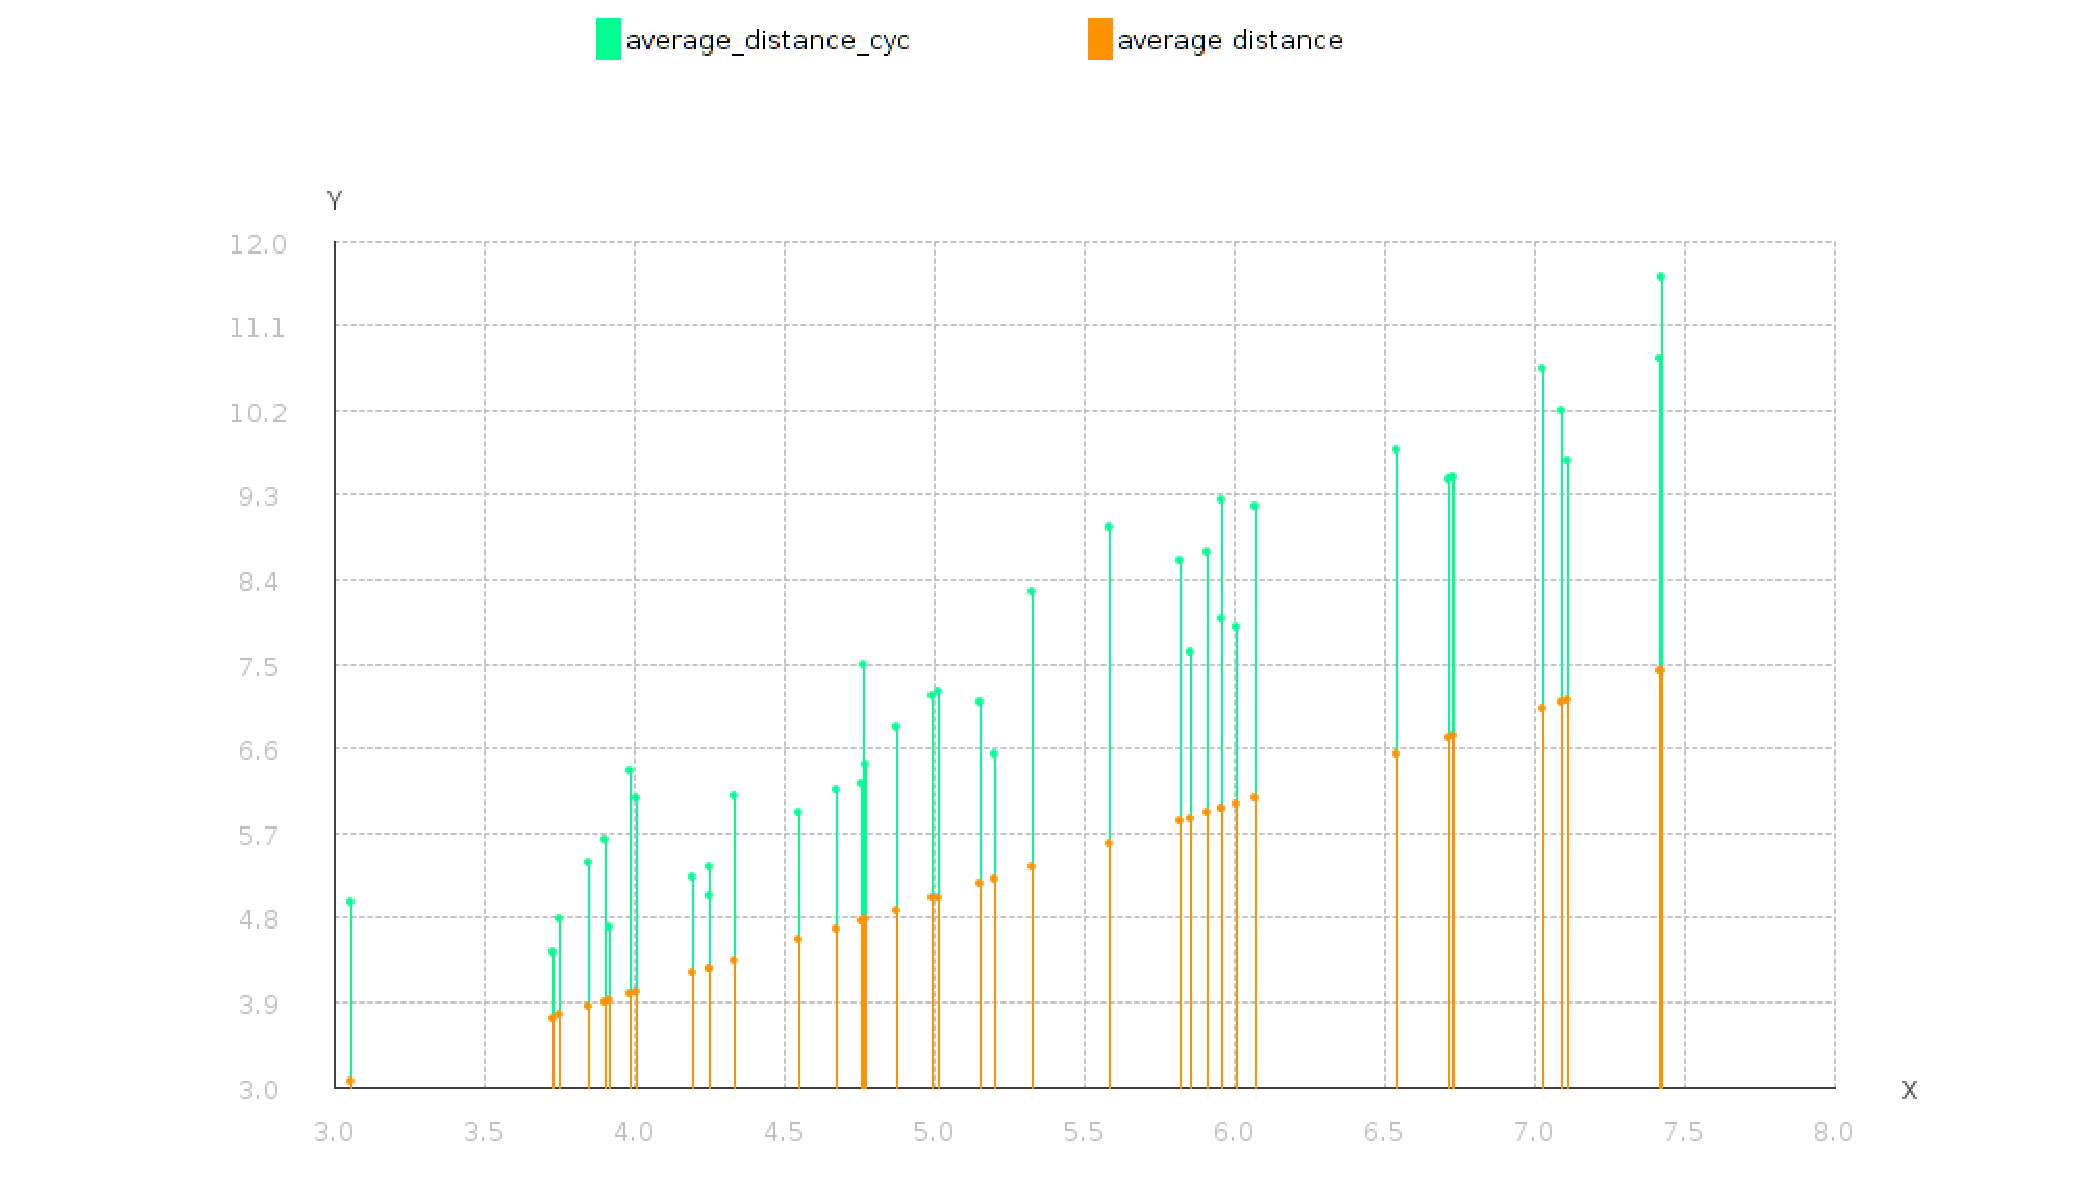
\includegraphics[width=1\textwidth]{Images/Chapter5/cyclic_vs_straightforward_avgdistance_n5_n8.eps}
  \end{center}
    \caption{average distance straightforward tour vs. average distance cyclic tour}\label{fig:avg_distance_cyclic_vs_avg_distance_forward}
\end{figure}

\subsection{Expected distance algorithm}\label{sec:test_expecteddistance}

Validation of backward expected distance algorithm comparing with the average expected distance of a tour $\tau$, where $\tau$ is assumed as a sorted permutation of the nodes, i.e. $\tau = (1,\ldots,n,0)$. The average expected distance is computed using monte carlo simulation under policy $\pi$ following $\tau$ and considering early replenishments defined by the policy.

\begin{figure}[!htbp]
  \begin{center}
   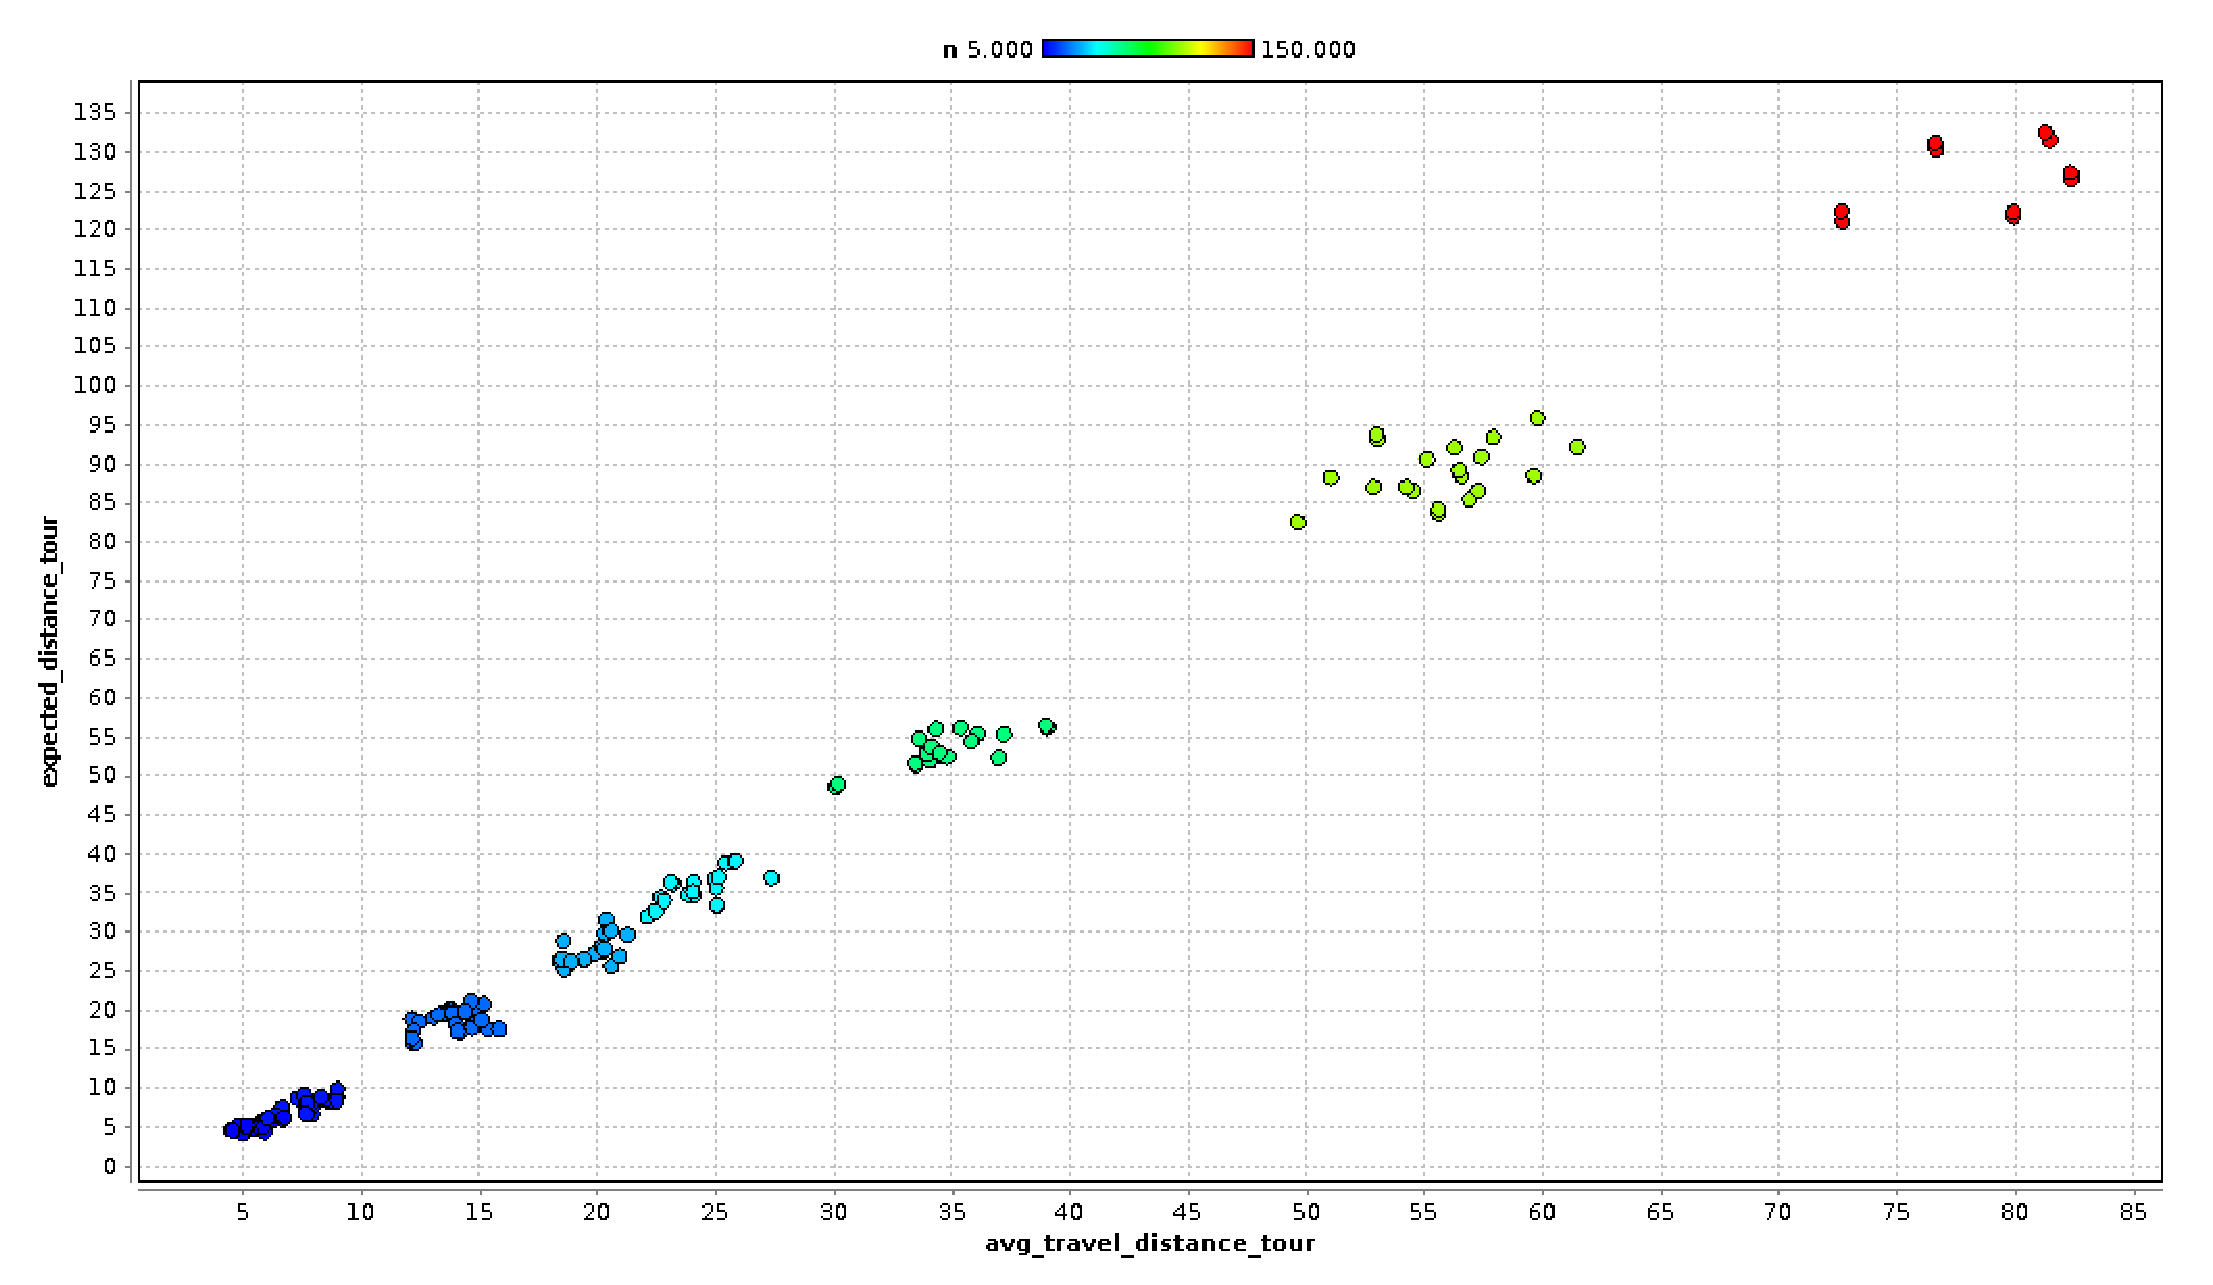
\includegraphics[width=1\textwidth]{Images/Chapter5/avg_vs_expected_distance_tour.eps}
  \end{center}
    \caption{average distance tour vs. expected distance tour}\label{fig:avg_distance_vs_expected_distance_tour}
\end{figure}

\begin{figure}[!htbp]
  \begin{center}
   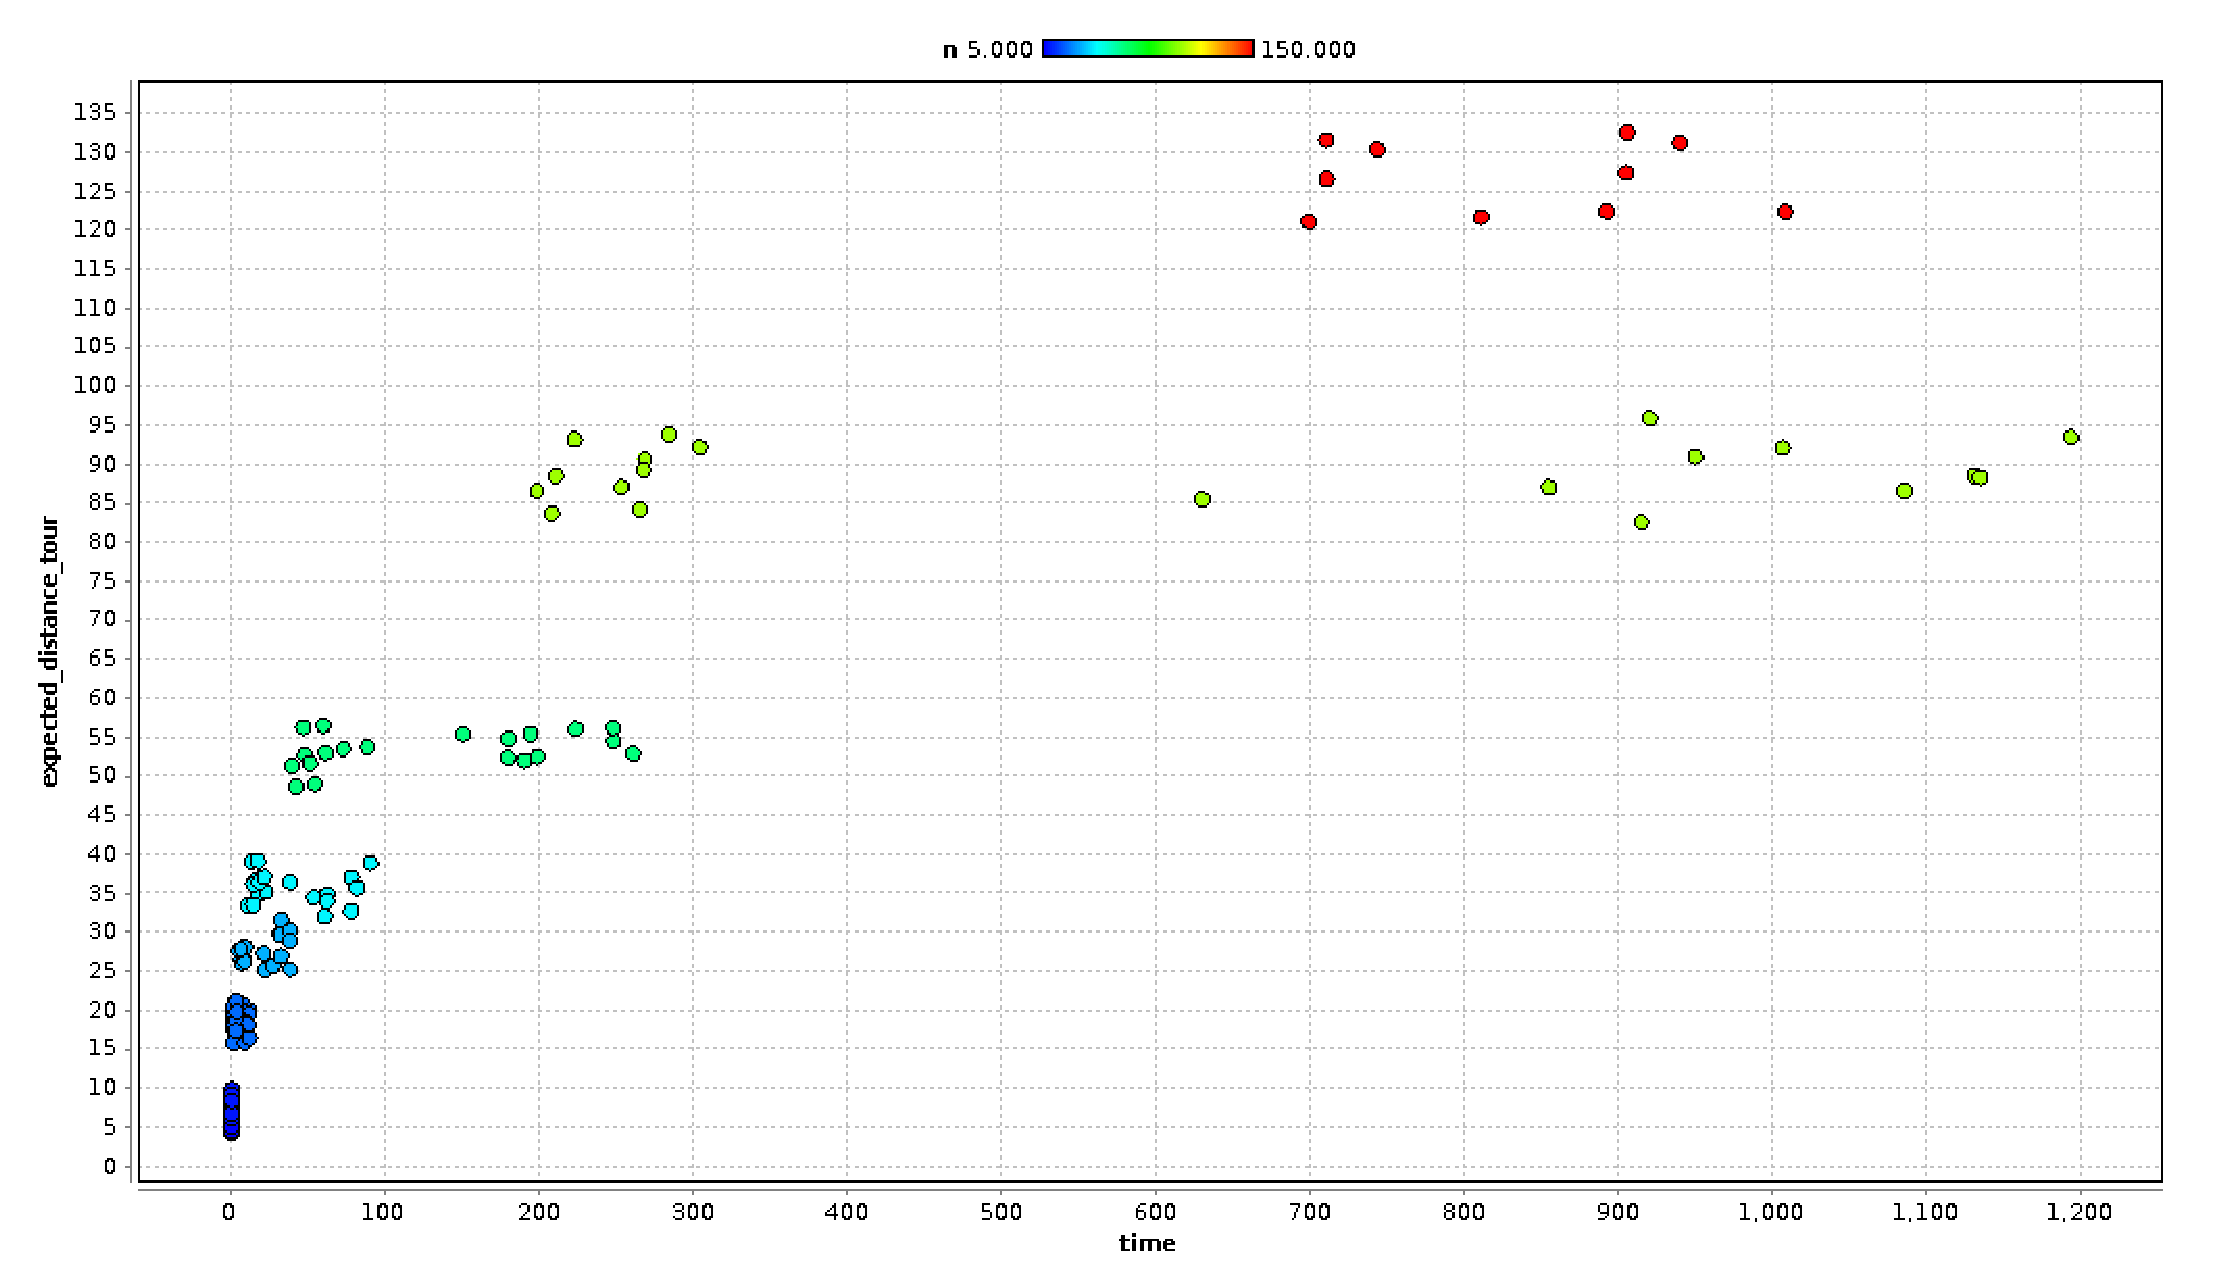
\includegraphics[width=1\textwidth]{Images/Chapter5/time_vs_expected_distance_tour.eps}
  \end{center}
    \caption{execution algorithm time vs. expected distance tour}\label{fig:time_distance_vs_expected_distance_tour}
\end{figure}